\documentclass{article}
\usepackage[utf8]{inputenc}

\title{Comparing House Prices in Different Neighborhoods of Toronto, Canada}
\author{Edison Murairi }
\date{June 2020}

\usepackage{natbib}
\usepackage{graphicx}

\begin{document}

\maketitle

\section{Introduction}
\subsection{Background}
Toronto will experience a rapid population growth over the next 20 years. Even worse, this growth is accelerating, and is expected to double by the year 2041 \cite{toronto}. This rapid increase in the population number significantly affects the real estate in Toronto, leaving the low-income households most vulnerable to inadequate housings or to a lack of any at all. \\

This challenge requires that the real estate industry adaptates  to the economic conditions of every social class in Toronto. Otherwise, it will not provide profitable and comprehensive service to meet this challenge. The first to do this is to understand the current real estate conditions in Toronto. Therefore, in this project, we will compare the house prices in neighborhoods of Toronto. \\

As this challenge will surely affect various areas - urban planning, environment, finance, etc. - the findings are intended to multiple stakeholders. These stakeholders who will benefit from these findings are the urban planning office of the Canadian government, the Ministery of environment, and also the real estate companies operating in the country.

\subsection{Problem Statement}
How does the price of houses vary between different neighborhoods of Toronto?

\subsection{Data}
This project requires first the housing price data. We have obtained house sales data of the Province Ontario \cite{houses_sale}. This dataset contains 6 columns: address, areaName (the name of the area where the house is located), the price, the latitude and longitude of the location. Figure \ref{fig:hs} shows an example of the house sales data.\\

\begin{figure}
	
	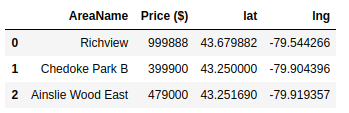
\includegraphics[]{hs.png}
	\caption{House Sales in the Ontario Province}
	\label{fig:hs}
	
\end{figure}

Secondly, we obtain venues data of each neighborhood from Foursquare using the postal codes obtained from the wikipedia page: "List of all Postal Codes in Canada M". From the Foursquare venues data, we will extract the neighborhood, the neighborhood latitude, the neighborhood longitude, the name of the venue, and the coordinates of the the venue (latitude and longitude)	Venue and the category of the venue. We will combine these informations with the the house sales data to compare how the price varies between neighborhoods of different characteristics. Figure \ref{fig:tv} shows an example of the venues data from Foursquare.

\begin{figure}[hbt!]
	
	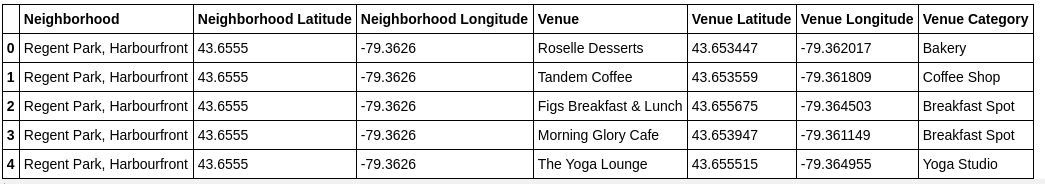
\includegraphics[width=\textwidth]{tv.png}
	\caption{Venues data in Toronto}
	\label{fig:tv}
	
\end{figure}

\section{Data Cleaning}

We obtained house sales data in the Ontario province from Kaggle \cite{houses_sale}. The dataset contains 25351 entries and 5 columns (Address, AreaName, Price, Latitude and Longitude). \\ 

Out of the 25351 entries, 483 or 1.9$\%$ of the dataset were missing AreaName. Because this is a small portion of the dataset, we remove all these rows with missing area names. Finally, we remove all the rows with a house outise Toronto. The final dataset hence obtained contains 5092 entries. Figure \ref{fig:final_hs} shows the first 3 rows of the final dataset. \\

\begin{figure}[hbt!]
	
	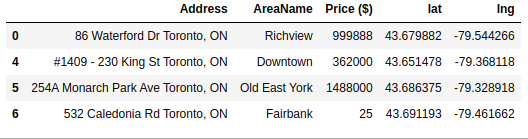
\includegraphics[width=\textwidth]{hs_final.png}
	\caption{Preview of the Toronto House Sales Dataset}
	\label{fig:final_hs}
	
\end{figure}

To obtain the venues data, we first scrapped the list of neighborhoods in Canada M and their postal codes from wikipedia. This list contains 180 entries, 77 of which have no assigned neighborhoods. We remove these entries fromt he dataset. To limit this list only to neighborhoods in Toronto, we remove all the entries where the borough does not contain the name Toronto. The final list contains 39 entries. We use the postal codes to retrieve the latitude and longitude of each location in the list. \\

We pass the coordinates of each region to the Foursquare API to retrieve venues data for the locations. We obtain 1535 entries, none of is missing values. Furthermore, all entries have the correct format. Hence no further processing was needed for this dataset. \\

The final step is to combine the housing price dataset with the venue dataset from Foursquare. In other words, we need to find the venues that are in the neighborhood of each house sold. To do this, we assign to each house a neighborhood of 0.015$^\circ$ Latitude wide, and 0.025$^\circ$ Longitude wide. %For example in Figure \ref{fig:region}, the red pin shows the location of the house and the square is the region we consider as its neighborhood. 
Then, for each house, we count the number of venue categories (Restaurant, Bakery, Spa, ...) falling into its neighborhood. An example of the final dataset that we will analyze is shown in Figure \ref{fig:final}.

\begin{figure}[hbt!]
	
	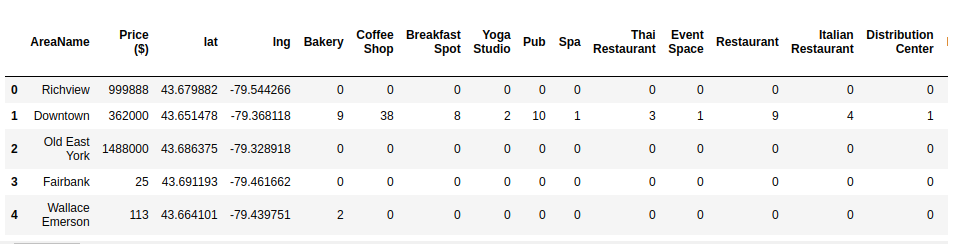
\includegraphics[width=\textwidth]{final.png}
	\caption{Preview of the Final Toronto House Sales Dataset}
	\label{fig:final}
	
\end{figure}

\section{Exploratory Analysis}

We first use Folium to visualize where the geographical distribution of the houses sold in Toronto, Figure \ref{fig:map1}. The orange marks represent the houses with price in the first quartile. The blue marks represent houses with prices in the second and third quartile. The red marks are the houses with prices above the third quartile. We observe that the houses in all three price ranges are distributed uniform across the city. 

\begin{figure}[hbt!]
	
	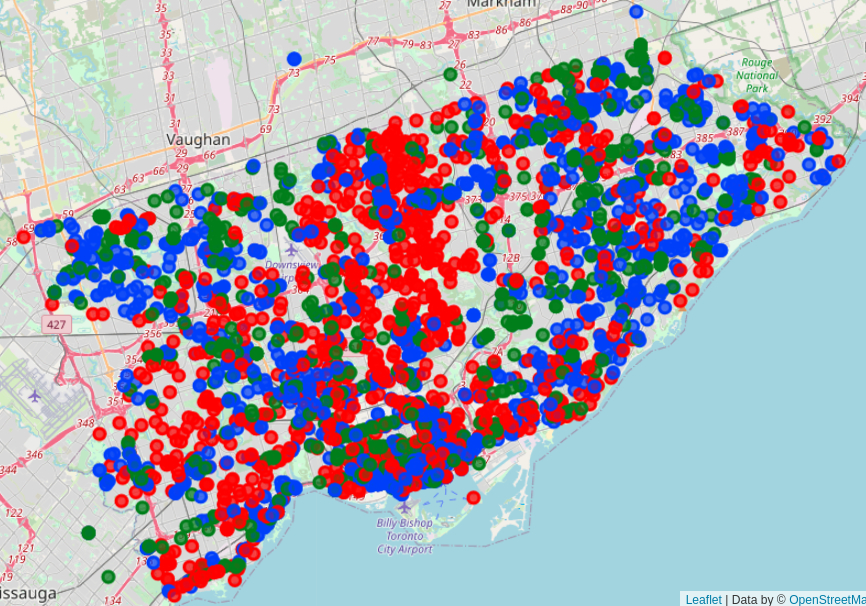
\includegraphics[width=\textwidth]{map1.jpg}
	\caption{Geographical Distribution of House Sales in Toronto. The orange marks represent the houses with price in the first quartile. The blue marks represent houses with prices in the second and third quartile. The red marks are the houses with prices above the third quartile.}
	\label{fig:map1}
	
\end{figure}

Next, we investigate the relation between the price of the house and the number of venues its neighborhood. Figure \ref{fig:vp} shows the plot of the price against the number of venues in its neighborhood. We can observe that the most expensive houses have the least venues around them. The price falls rapidly as the number of venues in the neighborhood increase. It is as if "rich" people live in places where they are "alone".

\begin{figure}[hbt!]
	
	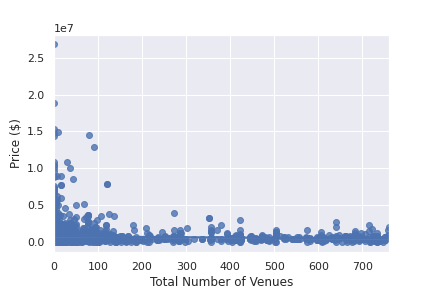
\includegraphics[width=\textwidth]{hp.png}
	\caption{Price of houses against the numbe of venues in the neighborhood}
	\label{fig:vp}
	
\end{figure}

\section{Analysis}

We have observed that the low price, medium price and high price houses are distributed uniformly across the city (Figure \ref{fig:map1}). We have also seen that the price falls off rapidly as the number of venues in the neighborhood increases. These two observations could be somewhat contradictory. To resolve this issue, we need a deeper analysis of how the price depends on the availability of venues in its neighborhood. We run a K-means clustering with 3 clusters to group houses with categories of different prices and different neighborhoods. \\

Figure \ref{fig:map2} shows the map of Toronto with the houses grouped in three diffferent clusters after the K-means clustering. The houses marked in red (first cluster) corresppond to the cheapest prices (price below 1.728 Million USD). The ones marked in green are the intermediate ones (price between 1.749 Million and 6.995 Million USD), and the ones marked purple are the most expensive ones (prices above). In the section below, we present the results in more details.

\begin{figure}[hbt!]
	
	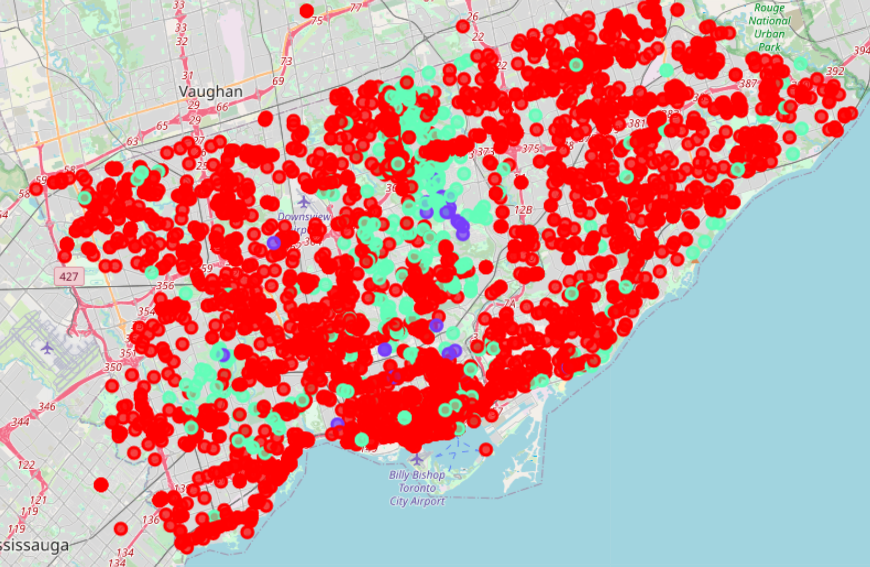
\includegraphics[width=\textwidth]{map2.png}
	\caption{Map of Toronto with Houses Grouped in 3 Clusters}
	\label{fig:map2}
	
\end{figure}

\section{Results}

From Figure \ref{fig:map2}, we can observe that the most expensive houses (purple) are in the middle of the city. The ceneter of Toronto is probably the most expensive one. Another observation is that most houses fall into lower price category, and are distributed almost everywhere. This consistent with the earlier observation that the houses were distributed quasi-uniformly across the city regardless of their prices. Another interesting feature is that the outskirt of the ciy has almost only the lower price category houses. Contrary to the uniform distribution claimed earlier, the medium price houses are mostly in the Central Western side of the city while the Eastern side mostly has the lower price ones. \\

Figures \ref{fig:hs1}, \ref{fig:hs2} and \ref{fig:hs3} show plots of the prices against the number of venues for the three different categories. We can see in each category that the price falls as the number of venues increases. Now, we investigate the distribution of venues in these three categories. From Figure \ref{fig:vp}, we expect that expensive houses will have fewer venues in their neighborhoods. 

\begin{figure}[ht]
	\begin{minipage}{0.3\linewidth}
		%\centering  % redundant
		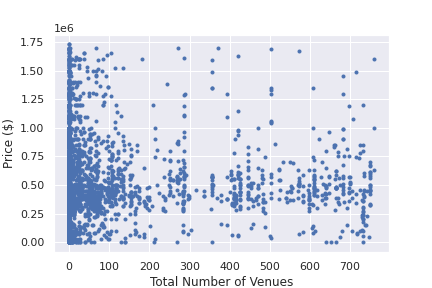
\includegraphics[width=\textwidth]{hs1.png}
		\caption{Category 1: Low Price}
		\label{fig:hs1}
	\end{minipage}%
	\hfill% not: "\hspace{0.5cm}"
	\begin{minipage}{0.3\linewidth}
		%\centering  % redundant
		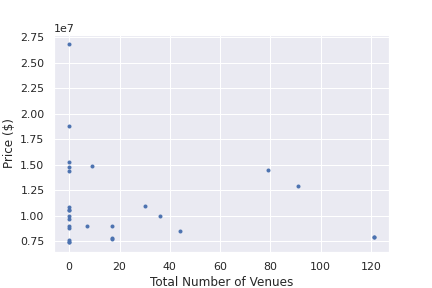
\includegraphics[width=\textwidth]{hs2.png}
		\caption{Category 2: Medium Price}
		\label{fig:hs2}
	\end{minipage}%
	\hfill% not: "\hspace{0.5cm}"
	\begin{minipage}{0.3\linewidth}
		%\centering  % redundant
		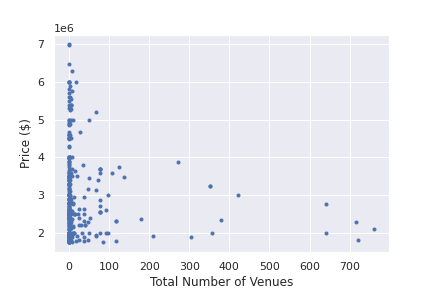
\includegraphics[width=\textwidth]{hs3.png}
		\caption{Category 3: High Price}
		\label{fig:hs3}
	\end{minipage}
\end{figure}

\begin{figure}[hbt!]
	
	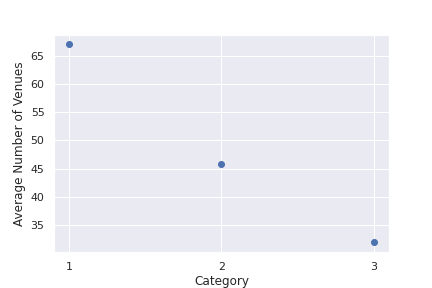
\includegraphics[width=\textwidth]{avg.png}
	\caption{Average Number of Venues against Price Category}
	\label{fig:avg}
	
\end{figure}

Figure \ref{fig:avg} shows the average number of venues in each category. We can see that the average falls linearly as we go through the categories. If we consider the category labels as the x-axis, we predict that the average number of venues as compared to the low prices, medium prices and high prices category follow a linear model with slope $-17.5$ and x-intercept $83.2$, or as given by the equation below:
\begin{equation}
	\textrm{Average Number of Venues} = -17.5\times \textrm{Price Category + 83.2}
\end{equation}
where the price category is an integer. Therefore, if we know the number of venues in the neighborhood, we can predict whether the house will be cheap, medium price or expensive.\\

\section{Conclusion and Recommendations}

In this exploratory analysis, we have studied how the price of houses vary in neighborhoods of Toronto. We have ran a K-means clustering with 3 clusters to group the houses in 3 price and neighborhood categories.  We have first found that the houses naturally fall into low, medium and high prices. The houses in the center of Toronto tend to be the expensive ones, suggesting that the center of Toronto is a rich area. The medium price houses tended to be in the West while the cheap houses are distributed across the entire city. Furthermore, most houses in the outskirt are the among the cheap ones. \\

Analyzing the distribution of the venues in the neighborhood of each house, we see that the number of venues falls rapidly as the number of venues increases. In other words, rich people live in areas where they are "alone". This suggests that most of venues in Toronto are probably small businesses. Furthermore, we derived a model to predict whether a given house is cheap, medium or expensive given the number of venues in its neighborhood. \\

In lights of these findings, we suggest further studies into the distribution of wealth and habitation in Toronto. This categorization could be the footprint of the social classes in the city. The future findings on the distribution of wealth will allow the city to provide affordable accomodation to most people in the future. This is crucial given that the population in Toronto is growing rapidly. Furthermore, we also see here an opportunity for employment research. It is important to confirm the types and wealth of businesses around the city since they seem related to the housing as shown in this study. Therefore, the city can understand what jobs they should provide to sustain its growing population.

\section{Acknowledgement}

We thank the Coursera IBM team for providing the training necessary to conduct this study through the Coursera Data Science Specializatio and Professional Certificate.


\bibliographystyle{plain}
\bibliography{references}
\end{document}
